\chapter{Integrationstests}

\section{Test 1 - Gleichm��iges Publizieren }
Dieser Test pr�ft, ob bei stetigem Publizieren die Frequenz korrekt bewertet wird und ob auf die Bewertung korrekt reagiert wird.

\begin{enumerate}
	\item Test-Launchfile starten:
	Mit \texttt{roslaunch arni\_core test\_1\_steady.launch} wird das Launchfile gestartet.\\
	Folgende Knoten werden dabei gestartet:
	\begin{verbatim}
	    countermeasure (arni_countermeasure/arni_countermeasure)
	    ninja_turtle (arni_core/predefined_subscriber.py)
	    node_manager (arni_nodeinterface/arni_nodeinterface)
	    processing (arni_processing/arni_processing)
	    steady_tree (arni_core/predefined_publisher.py)
	\end{verbatim}
	Debei besteht folgende Verbindung der Knoten (Debugging-Knoten zur �bersichtlichkeit ausgenommen):\\

\begin{figure}[htbp]
    \begin{minipage}[t]{16cm}
        \vspace{0pt}
        \centering
        
\includegraphics[scale=0.3]{./bilder/integrationstests/test_1_nodegraph.png}
        \caption{steady\_tree publiziert mit 100Hz auf /forest, ninja\_turtle abonniert forest.}
    \end{minipage}
    \hfill
\end{figure}  

    Die Frequenz von /forest wird unter 80Hz als LOW und �ber 120Hz als HIGH bewertet.
    Der Countermeasure-Knoten hat das Constraint alle 10 Sekunden \textit{frequency of forest is ok} auszugeben, falls die Frequenz mit OK bewertet wurde.

\newpage
	\item �ffnen der GUI:
	In die Konsole wird \texttt{rosrun rqt\_gui rqt\_gui} eingegeben und ausgef�hrt.\\
	\item �ffnen der Widgets:
	Ausw�hlen des Widgets \textit{Logging > Console},\\
    Debug Messages ausblenden\\

\begin{figure}[htbp]
    \begin{minipage}[t]{16cm}
        \vspace{0pt}
        \centering
        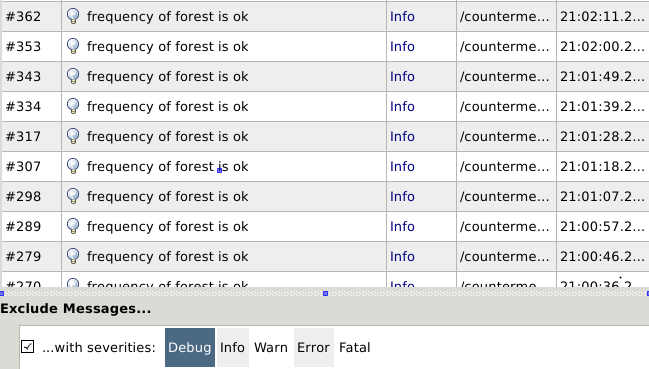
\includegraphics[scale=0.5]{./bilder/integrationstests/test_1_rqt_freq_ok.png}
        \caption{steady\_tree publiziert mit 100Hz auf forest. ninja\_turtle h�rt zu.}
    \end{minipage}
    \hfill
\end{figure}  


    Es ist zu sehen, dass die Nachricht des Countermeasure-Knotens alle 10 Sekunden publiziert wird.
\end{enumerate}